%
%  Vorlage/Template fuer #EBT
%
%  Created by Prof. Dr. Detlef Kreuz on 2010-08-14.
%  Copyright (c) 2010 . All rights reserved.
%
\documentclass[12pt,toc=bib,toc=listof]{scrreprt}
\usepackage[ngerman]{babel} 
\usepackage[utf8]{inputenc}
\usepackage[T1]{fontenc}
\usepackage{lmodern}
\usepackage{setspace}

\usepackage{hyperref}
\hypersetup{
  ,colorlinks=true
  ,linkcolor=blue
  ,citecolor=blue
  ,filecolor=blue
  ,urlcolor=blue
  }

%%%%%%%%%%%%%%%%%%%%%%%%%%%%%%%%%%%%% % (fold)
% Vom Studierenden zu aendernde Werte
\newcommand{\ebttopic}{Docker}
\newcommand{\ebtstudentname}{Jerome Tagliaferri}
\newcommand{\ebtstudentid}{190530}
\urldef{\ebtstudentmail}\url{jtagliaf@stud.hs-heilbronn.de}
%
%%%%%%%%%%%%%%%%%%%%%%%%%%%%%%%%%%%%% % (end)

\usepackage{ifpdf}
\ifpdf
\usepackage[pdftex]{graphicx}
\else
\usepackage{graphicx}
\fi

\graphicspath{{images/}}
\usepackage[headsepline]{scrpage2}
\pagestyle{scrheadings}
\clearscrheadfoot
\ihead{Fallstudie Entwicklungswerkzeuge: \ebttopic}
\ohead{\pagemark}
\renewcommand*{\chapterpagestyle}{scrheadings}
\renewcommand*{\chapterheadstartvskip}{}

\titlehead{\flushright
%\includegraphics{HHN_KOMPLETT_4C.jpg}

\includegraphics[scale=0.6]{HHN_ab_40_mm_4c_neg.png}
}
\subject{Fallstudie Entwicklungswerkzeuge (281761)}
\title{\ebttopic}
\author{\ebtstudentname\footnote{\ebtstudentid, \ebtstudentmail}}
%% Datum nie auf einen festen Wert setzen
\publishers{Eingereicht bei Paul Lajer}

%\pagestyle{headings}

\begin{document}
\pagenumbering{roman} 
\selectlanguage{ngerman}
\maketitle
\tableofcontents

\addchap{Abkürzungsverzeichnis} % (fold)
\label{sec:abkuerzungsverzeichnis}

\begin{description}
  \item[ABK:] ABKÜRZUNG 
\end{description}

% chapter abkuerzungsverzeichnis (end)

\listoffigures
\listoftables

\onehalfspacing
\newpage
\pagenumbering{arabic}

\chapter{Einleitung} % (fold)
\label{sec:einleitung}

\section{Motivation} % (fold)
\label{sec:motivation}

Technologien welche im Big Data und Cloud Umfeld entstanden und gewachsen sind, werden immer häufiger auch in anderen Bereichen eingesetzt. So entstand die Virtualisierung von Betriebssystemen als Grundlage des Cloud Computing um auf individuelle Wünsche und eine stetig schwankende Ressourcenverteilung zu reagieren. So wie diese Technology ihren Weg in viele weitere Bereiche geebnet hat, findet die Container Virtualisierung eine immer vielseitigere Anwendung.
Getragen und weiterentwickelt von Branchengrößen wie Google oder IBM ist die Container Virtualisierung momentan eine der sich am schnellsten wachsenden Bereiche der Informatik.
Sie verspricht eine noch stärkere flexibilität und automatisierung von Systemen und Ressourcen und ist deshalb ein relevantes Thema für jede Branche, welche mit Soft- und Hardwaresystemen in Kontakt kommt.


% section motivation (end)

\section{Ziel der Arbeit} % (fold)
\label{sec:ziel_der_arbeit}
Diese Ausarbeitung soll als Einstieg in den Bereich Container Virtualisierung dienen und dabei Docker als zentrale Komponente behandeln und vorstellen.
Es soll ein umfassender Einblick in die Thematik und deren unterschiedliche herangehensweisen erörtert werden, wodurch eingeschätzt werden kann, inwieweit sich die Container Virtualisierung für individuelle Einsatzzwecke eignet.

% section ziel_der_arbeit (end)

\section{Vorgehensweise} % (fold)
\label{sec:vorgehensweise}

Um dieses Ziel zu erreichen, werden die Grundlagen in Form der Idee und grundlegenden Historie und deren Konzepte, welche die Basis von Docker beinhalten, erläutert.
Daraufhin wird die Umsetzung dieser Konzepte und deren Erweiterungen in Docker betrachtet und daraus auf mögliche Vor- und Nachteile geschlossen.
Aufbauend auf diesen Grundlagen, werden Anwendungsbereiche vorgestellt, in dennen Docker in einem produktiven Umfeld eingesetzt wird und welche Tools den massiven und verteilten Einsatz von Containern erleichtern.
Mögliche Alternativen und deren Unterschiede, sowie ein Ausblick in die Zukunft der Container Virtualisierung sollen diese Arbeit abrunden.



% section vorgehensweise (end)
% chapter einleitung (end)

\chapter{Docker Grundlagen} % (fold)
\label{sec:grundlagen}

\section{Was ist Docker ? Was versteht man darunter ?}
Die Bezeichnung Docker, findet schon lange nicht nur im Cloud spezifischen Umfeld erwähnung.
Der aufmerksame Nutzer stößst immer öfter schon bei der Installation von Anwendungen auf diesen Term.
Ein Beispiel hierfür wäre das Test und Entwicklungswerkzeug Jenkins, welches nun an erster Stelle die Option eines Docker Containers als mögliche Installationsquelle zur Verfügung stellt. \cite{jenkins}
Viele weitere Hersteller welche Werkzeuge anbieten, welche auf unterschiedlichste Bibliotheken und Anwendungen angewiesen sind, greifen immer öfter zu Docker. 
Hierbei stellt sich jedoch die Frage, was ist Docker ? \\
Auf der Offiziellen Seite wird diese Frage mit folgendem Satz beantwortet :

\begin{quote}
	\footnote[1]{Vgl. https://www.docker.com/what-docker}
	"`\textit{Docker is the world's leading software containerization platform}"
\end{quote}
Da diese Aussage wenig bis keinen Informationsgehalt bietet, macht es sinn, sich zuerst einmal die Grundlegenden Konzepte und historische Entwicklung der Container Virtualisierung anzuschauen. 

\section{Die Geschichte, der Ursprung und Entwicklung von Docker}
Wie so viele Entwicklungen im technischen Umfeld sind die Konzepte und ersten Umsetzungen der Container Virtualisierung schon weitaus älter als man vermuten sollte.
Es begann alles mit der Idee Services untereinander und vom eigentlichen Host isolieren zu können.
Dieses Konzept wurde erstmals im Jahre 1979 unter UNIX mit der funktion des "chroot" umgesetzt, diese Funktion isolierte das Hauptverzeichnis eines Prozresse an einem neuen Ort.\\
Erst im Jahre 2000 wurde diese Funktionalität unter FreeBSD mit dem Namen Jails erneut aufgenommen und erweitert.
Diesmal konnte nicht nur das Dateisystem isoliert werden, sondern auch dazugehörige Benutzer, Netzwerk und dazugehörige Prozesse.\\
Über die nächsten acht Jahre können viele weitere Technologien gefunden werden, welche diese Funktionalitäten integrieren. Darunter 
Linux VServer, Oracle Solaris Zones, OpenVZ, Process Container (von Google entwickelt),ControlGroups im Linux Kernel und WPARS.
2008 entstand dann durch die Entwicklung bei IBM  das Linux Containers project (LXC) welches die unterschiedlichsten Technologien im Container Umfeld zusammen brachte und somit die vollständigste Implementierung eines Linux Container Managements darstellte.
Die besonderheit von LXC, bestand darin, dass es seine ressourcen komplett aus dem Linux Kernel bezog ohne zusätzliche Software zu benötigen.
Am 15.03.2013 wurde Docker, durch den dotCloud Gründer Solomon Hykes zum ersten mal der Öffentlichkeit vorgestellt.
Diese Vorstellung bestand nur aus einem fünf minütigen Vortrag auf der Python Entwickler Konferenz in Kalifornien.
Verbreitete sich jedoch weltweit mit enormer Geschwindigkeit wodurch das Projekt schnellstmöglich auf GitHub offen gelegt wurde um die weitere Entwicklung voran zu treiben.

\section{Wie funktioniert Docker ?}

Abgesehen von der schnellen Verbreitung von Docker, war vielen Interessenten die eigenltiche Funktionsweise nicht vollständig bewusst.
Docker versprach, ein Stück Software in ein komplettes Dateisystem zu verpacken, welches alles beeinhaltete was für das Ausführen dieser  nötig ist. Dazu gehört der Quellcode, System Bibliotheken/Tools und die Ausführumgebung. Dies sorgte dafür, dass sich die Software immer gleich verhält egal auf welcher Umgebung sie ausgeführt wird. 
Hinzu kam, das Container aufgrund ihrere Größe und Isolation  beliebig gestartet oder gestoppt werden konnten, ohne das Host System zu beeinflussen.
Einige dieser Eigenschaften, werden oftmals sehr gerne mit denen Virtueller Maschinen verglichen, da es auf den ersten Blick sehr viele Ähnlichkeiten aufweist.
Die Entwickler von Docker, distanzieren sich jedoch sehr klar von diesem Vergleich und machen darauf aufmerksam, dass Docker sehr viel mehr ist.
Um jedoch die Grundlegenden funktionsweisen zu erläutern, macht es Sinn diesen Vergleich zu bemühen.

\begin{figure}
	\centering
	\caption{VM vs Container}
	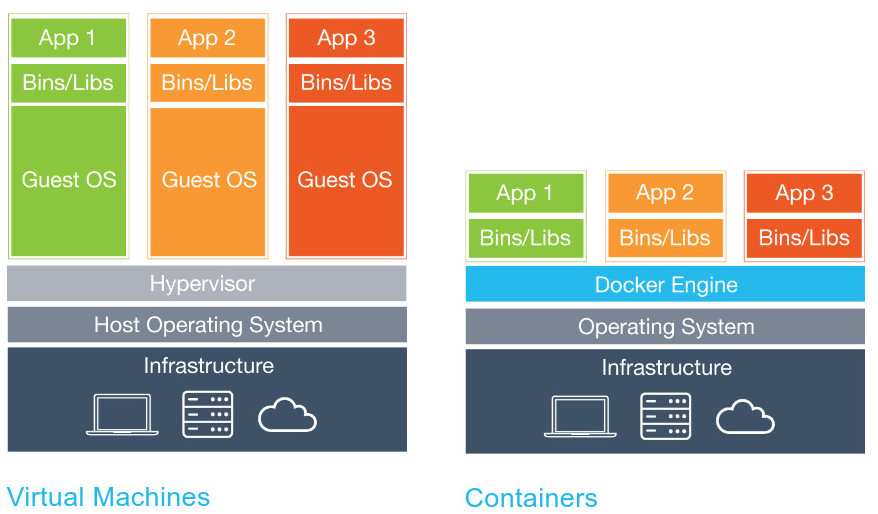
\includegraphics[width=15cm, height=8cm, scale=0.3]{dockerVM.jpg}
	Quelle: www.docker.com/what-docker
\end{figure}

Wie in der Abbildung unschwer zu erkennen, liegt ein sehr wesentlicher Unterschied in der größe der Lösungen.
Da eine Virtuelle Maschine über einen Hypervisor mit dem Hostsystem kommuniziert bringt es bei jeder Instanz ein komplettes Gast Betriebssystem mit sich. Dies führt dazu, dass nur wenige Instanzen auf einem Host ausgeführt werden können.
Da jedoch jeder Docker Container den Kernel des Hostsystems nutzt, ist es möglich auf einer Maschine mehrere hundert Container parallel zu betreiben.
Damit dies möglich wurde, nutzt Docker mehrere Funktionen des Linux Kernels wobei folgende essentiell sind:

- CGroups : Limitiert und verwaltet die Ressourcen wie CPU , Arbeitsspeicher, Netzwerk und Festplattenzugriff welche einer Prozessgruppe zugewiesen werden können. 

- Namespace isolation : Prozessgruppen sind nicht in der Lage die Ressourcen anderer Gruppen zu sehen.

\begin{figure}
	\centering
	\caption{Treiber}
	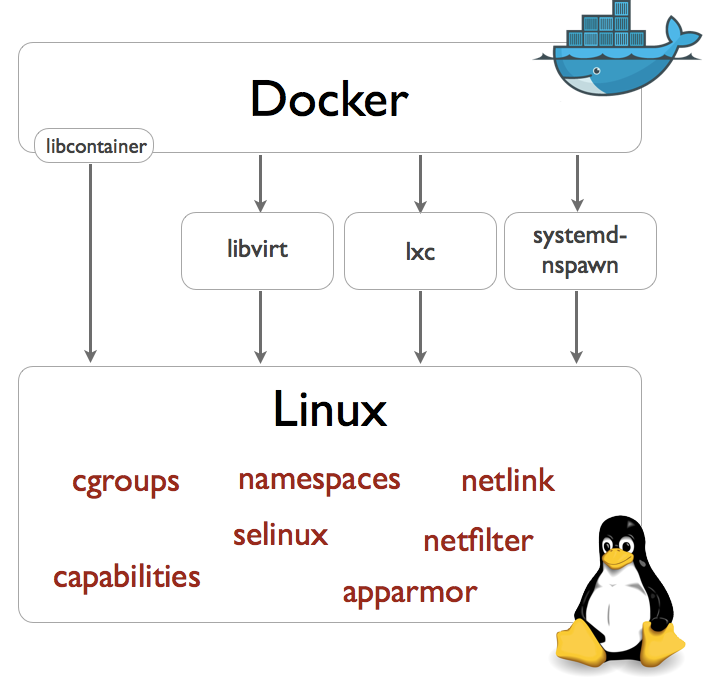
\includegraphics[width=15cm, height=8cm, scale=0.3]{docker-execdriver-diagram.png}
	Quelle: http://jancorg.github.io/blog/2015/01/03/libcontainer-overview/
\end{figure}

Bis zur Version 0.9 war Docker von der LXC-Bibliothek abhängig, nutzte jedoch ab diesem Zeitpunkt eine eigens Entwickelte Bibliothek namens libcontainer.
Diese neue Bibliothek wurde entwickelt um weitere Isolationstechnologien zu nutzen außerdem war Docker nun in der Lage alle nötigen Komponenten aus einer Hand zu bieten.
Dies gab auch Microsoft die möglichkeit Docker unter Windows lauffähig zu machen da alle Komponenten veröffentlicht wurden und allgemein als Standard angesehen werden.
Eine weitere sehr essentielle Komponente stellt UnionFS dar.
Dies ist ein Dateisystem, welches die Fähigkeit besitzt unterschiedliche Schichten (Standorte) von Dateien zu bündeln und einem Prozess zur Verfügung zu stellen.
In Docker wird dies genutzt, um nur neue oder veränderte Dateien dem Container Verfügbar zu machen um so die Geschwindigkeit zu erhöhen und beim Einsatz von großen Mengen an Containern Speicherplatz zu sparen.


\section{Welche Funktionen enthält Docker /Docker Workflow ?}
Aufbauend auf diesen Grundlagen, soll nun eine mögliche Vorgehensweise erläutert werden, welche den Einsatz von Containern beschreibt.
Zuerst sollten jedoch die einzelnen Komponenten vorgesetellt werden :

\begin{itemize}
	\item \textbf{Docker daemon}: Docker nutzt eine Client-Server Architektur wobei der Daemon einen Serverseitigen Prozess darstellt, welcher die Aufgabe hat Container zu erstellen, auszuführen und zu verteilen.
	
	\item \textbf{Docker CLI}: Der Docker Client hat die Möglichkeit über eine REST API mit dem Docker daemon zu kommunizieren und Befehle zu übermitteln.
	
	\item \textbf{Docker Image Index}: Ein öffentliches oder Privates Verzeichnis über alle Docker Images welche vorhanden sind. Möchte man ein Image ausführen, wird meist zuerst lokal nach solchem gesucht, sollte der Prozess nicht fündig geworden sein, wird im Docker eigenen Repository DockerHub weiter gesucht, welche sehr viele spezielle Images anbietet.\\
	
	\item \textbf{Docker Containers}: Ein Container, welcher sich meist aus mehreren Images zusammen stellt. Diese enthalten alle nötigen Bibliotheken/Tools und Quellcode um die Applikation auszuführen.
	Wenn ein solcher Container angelegt wird, wird wie in Abbildung 2.3 zu sehen ein neuer Layer angelegt. Dieser kann dann später alle Veränderungen aufnehmen.
	
	\item \textbf{Docker Images}: Stellt ein Dateisystem mit verschiedenen Parametern dar welches nur gelesen aber nicht beschrieben werden kann.
	
	\item \textbf{Dockerfiles}: Skripte welche den Bau eines Images vereinfachen und automatisieren.
\end{itemize}

\begin{figure}
	\centering
	\caption{Container-Images}
	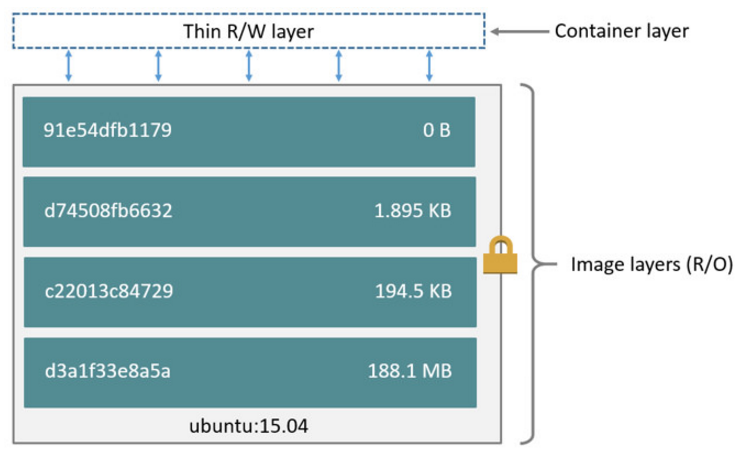
\includegraphics[width=15cm, height=8cm, scale=0.3]{container-images.png}
	Quelle: https://docs.docker.com/engine/userguide/storagedriver/imagesandcontainers/
\end{figure}

Das zusammenspiel dieser Komponenten, sorgt dafür, dass die Erstellung , Ausführung und Administration von Docker Containern sehr schnell und einfach funktioniert.
Dies soll nun anhand einer Webapplikation verdeutlicht werden.
Hierführ gehen wir davon aus, dass Docker bereits installiert und wir  eine  simple "Hello World !" Django Applikation erstellt haben.
Diese nutzt folgende Technologien : Python 3 mit Django und Gunicorn als Web Server.

1. Um die Erstellung des Containers zu erleichtern, wird im Hauptverzeichnis der Applikation eine requirements.txt angelegt welche unsere Bedingungen enthält.\\
In diesem Fall :

Django==1.9.4
gunicorn==19.6.0

2. Nun soll ein script erstellt werden, welches später die richtige Ausführung des Web Servers übernehmen soll.
Hierzu wird eine start.sh Datei erstellt welche folgenden Inhalt besitzt :

\#!/bin/bash\\
exec gunicorn helloworld.wsgi:application \ \\
--bind 0.0.0.0:8000 \ \\
--workers 3 \\ 

Über den exec Befehl wird hierbei Gunicorn mit unserer helloworld applikation gestartet, welche wir über die lokale Adresse 0.0.0.0 und den Port 8000 ansprechen wollen. Zur Sicherheit und verbesserten Bearbeitung von anfragen werden zusätzlich drei "Arbeiter" erstellt.

3. Es kann damit begonnen werden eine Dockerfile im Hauptverzeichnis zu erstellen welche unterschiedliche Befehle beinhalten kann, um die Umgebung anzupassen.

\# Nutzt ein vorgefertigtes Python3 Image von DockerHub als Basis
FROM python:3-onbuild

\# Kopiert den Inhalt des Verzeichnises an die angegebene Stelle innerhalb des Containers 
COPY . /usr/src

\# Öffnet den Port 8000 um eine Kommunikation zu ermöglichen
EXPOSE 8000

\# führt das Skript des Web Servers aus
CMD ["usr/src/start.sh"]

4. Das Image muss nun über folgenden Befehl gebaut werden :

sudo docker build -t helloworld .

Dies führt docker mit root rechten aus um innerhalb des momentanen Verzeichnisses die Dockerfile abzuarbeiten und einen Container mit dem namen helloworld zu erstellen.

5. Als letzter Schritt muss der Container über das Terminal gestartet werden :

sudo docker run -it -p 8000:8000 helloworld

Dies führt den Docker Container helloworld aus und verbindet sich über den Port 8000 mit dem Web Server.

Werden nun Änderungen an der Applikation vorgenommen müssen nur noch die letzten zwei Schritte ausgeführt werden.
Hierdurch können Neuerungen an Software Systemen sehr schnell umgesetzt und in Betrieb genommen werden ohne mit Komplikationen konfrontiert zu werden.
Dieses kleine Beispiel kann nicht alle Funktionalitäten von Docker umfassen, gibt aber einen ersten Einblick in die Arbeit mit Containern.
Ansatzpunkte welche das dargestellte Beispiel erweitern , sind die Verlinkung von Containern (sollte z.b. eine Datenbank hinzukommen) oder auch das erstellen von eigenen Basis Images welche dann veröffentlicht und verteilt werden können.

\section{Vorteile und Nachteile von Docker}

% chapter grundlagen (end)

\chapter{Docker im Produktiveinsatz}

\section{Anwendungsbereiche - Wer nutzt Docker ?}

\section{Tools - Kubernetes / Docker Swarm}


\section{Alternativen und Unterschiede ?}

\section{Wieso gerade Docker ?}

\section{Weshalb kommt der Durchbruch erst jetzt ?}

\chapter{Fazit - Ausblick} % (fold)
\label{sec:fazit}
Im Schlusswort / Fazit („Was ich gesagt habe und was daraus folgt“) kann ein kurzer
Rückblick auf das Thema erfolgen. Wenn das Thema dies zulässt, können auch Zu-
kunftsperspektiven aufgezeigt und höchst subjektive Bewertungen des Verfassers ein-
gebracht werden.
- Wie soll es weiter mit Docker gehen, was sagt der momentane Plan ? ( Roadmap )

% chapter fazit (end)

\appendix
\begin{thebibliography}{99}
\raggedright
%%% Printquellen zuerst
%%% Beispiel
\bibitem{Th11} Manuel René Theisen:
 \emph{Wissenschaftliches Arbeiten: Technik -- Methodik -- Form};
 15.~Auflage; Vahlen; München 2011;
 ISBN 978-3-8006-3830-7

%%% Internetquellen: Beispiel
\bibitem{hhneb} \emph{Hochschule Heilbronn};
 \url{http://www.hs-heilbronn.de/};
 abgerufen am 14.08.2010
 
\bibitem{jenkins} \emph{Jenkins};
 \url{https://jenkins.io/};
 abgerufen am 02.12.2016
 
\bibitem{dockerWhat} \emph{Docker};
 \url{https://www.docker.com/what-docker};
 abgerufen am 02.12.2016

 
 
 
 
 
 
\end{thebibliography}
\end{document}

